\subsection{Application overview}

This section covers a more detailed description of the application's web interface and describes different actions, which can be performed by interacting with the application.

\subsubsection{Posting an advertisement}

\paragraph{Step 1 - Generating an account an logging in}

Account generation and logging in forms are accessed from the homepage. An account is generated from a random seed (fetched from the Wordnik API \citep{wordnik}), which can be updated by triggering the refresh button. The algorithm behind address and encryption key generation allows for regeneration of the private key by providing that seed. Thus, the seed needs to be safely stored by the user in order to be able to gain access to the account in case of password being hacked, or forgotten. The password needs to be strong enough and contain at least 8 characters, out of which at least one letter and number. Account needs to be configured with the user's real name and residential address, which will safely be stored and only used for logistics purposes. Once the account created, user may log in to the application by providing the address and the password.

\begin{figure}[H]
\centering
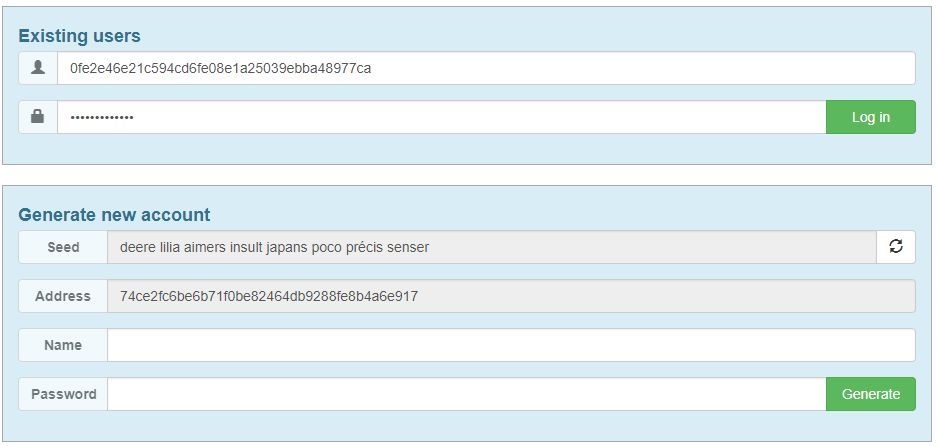
\includegraphics[scale=0.56]{app_screens/login.png}
\caption{Homepage of the web interface.}
\label{fig:applogin}
\end{figure}

\paragraph{Step 2 - Defining item details}

Once logged in, an advertisement can be submitted by triggering the button, which is located on the top-right corner of the interface (on the navigation bar). First step of configuring an advertisement involves definition of the item, which is to be sold, using the application. Item is defined by its title, description and an image. Once the form is completed, the user may move to the next step. In order to simplify the implementation process, the images are provided by including links to their corresponding address on the web.

\begin{figure}[H]
\centering
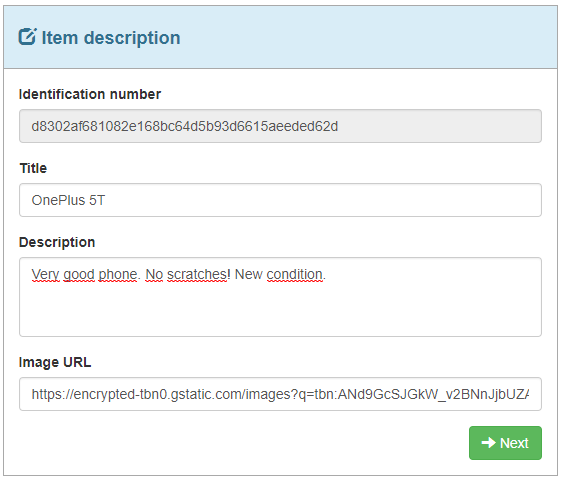
\includegraphics[scale=0.48]{app_screens/new_item_1.png}
\caption{First step of configuring an advertisement.}
\label{fig:newitem1}
\end{figure}

\paragraph{Step 3 - Defining initial terms}

Seller is required to define initial terms, which will be visible to potential buyers. Those terms consist out of the price, shipment deadline and sensor configuration. Sensors are configured with threshold values and binary (yes or no) inclusion parameters. Once all of the parameters are filled in, the advertisement is ready to be submitted and added to the database.

\begin{figure}[H]
\centering
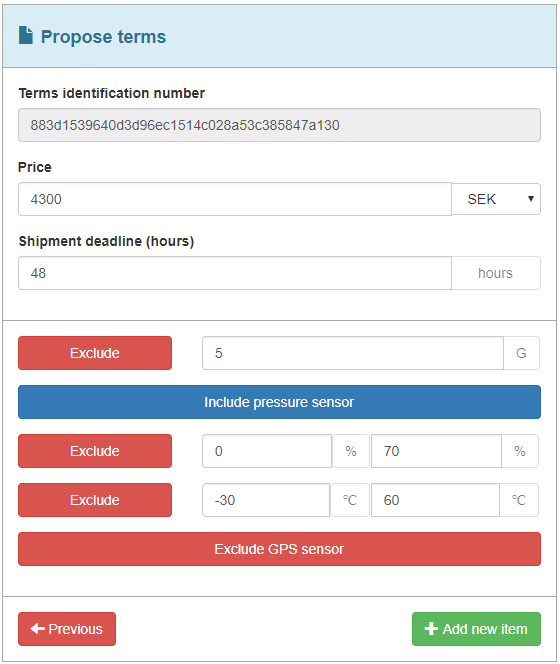
\includegraphics[scale=0.48]{app_screens/new_item_2.png}
\caption{Second step of advertisement configuration.}
\label{fig:newitem2}
\end{figure}

\subsubsection{Proposing terms for an advertisement}

\paragraph{Step 1 - Browsing advertisements}
Assuming that the user is logged in to the application, the advertisement browser page may be accessed in order to find an item that is interesting to the user. Once an item of interest is located, it can be clicked, in order to open the advertisement information window, which also provides functionality of proposing terms.

\begin{figure}[H]
\centering
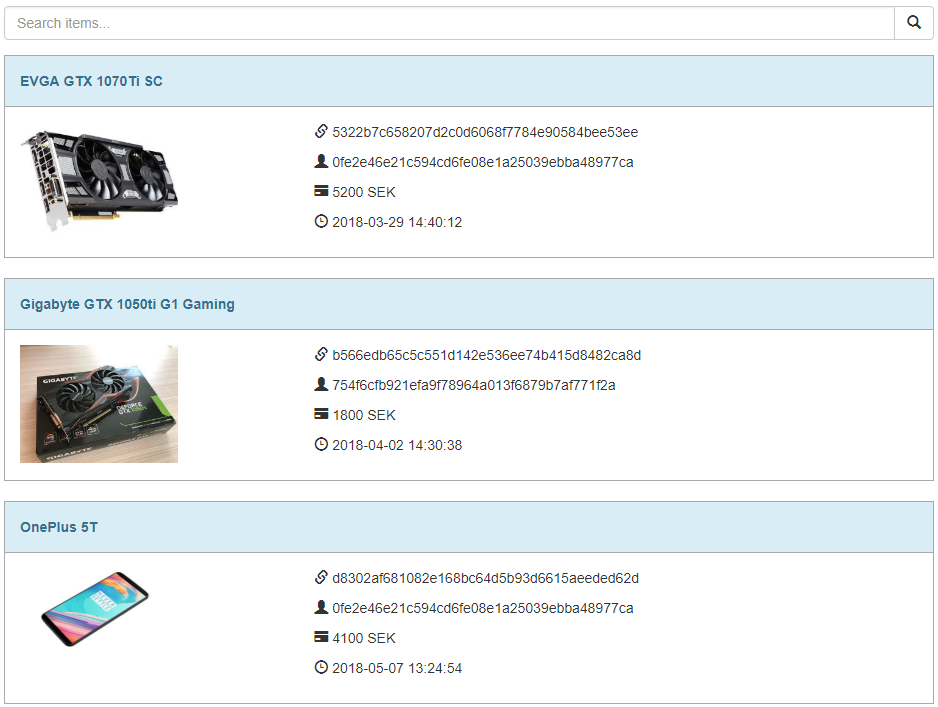
\includegraphics[scale=0.59]{app_screens/item_browser.png}
\caption{Advertisement browser page.}
\label{fig:itembrowser}
\end{figure}

\paragraph{Step 2 - Proposing terms}

Once the advertisement information page is accessed, user can propose own terms by clicking the button below the initial terms display. That triggers a modal, which has roughly the same appearance as shown in Figure \ref{fig:newitem2}. The contents of the modal are preconfigured with the initial terms for that particular advertisement and can be changed to other values, if so desired. Terms, which are added by potential buyers, are visible to everyone. This allows for a bidding auction-like functionality, which benefits the sellers.

\begin{figure}[H]
\centering
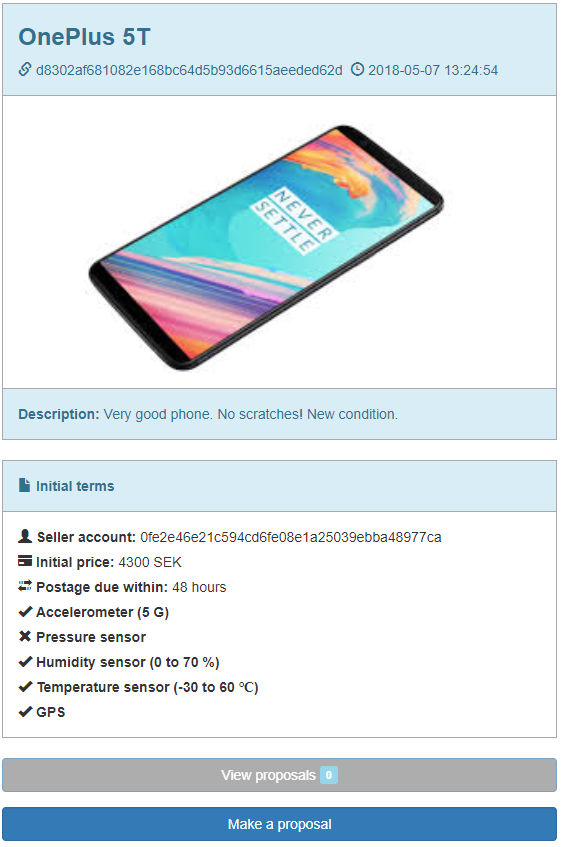
\includegraphics[scale=0.58]{app_screens/item_display.png}
\caption{Page that displays an advertisement in detail.}
\label{fig:itemdisplay}
\end{figure}

\subsubsection{Initiating an agreement} \label{section:initiation}

\paragraph{Step 1 - Locating the advertisement}

An agreement is initiated when the seller accepts a proposal for a given advertisement. This is achieved through navigating to the submenu of the item manager module, called "My adverts", which is located in the dropdown menu of the top navigation bar (menu is dropped down by clicking the "Item manager" button). This allows the user to browse his/her own submitted advertisements. The next step is to find the advertisement in question in the advertisement list.

\paragraph{Step 2 - Browsing and accepting terms}

Once the advertisement is located, seller can browse through proposed terms of that agreement by clicking "Manage proposals" button. Terms can be organized, according to their status. In order to accept the terms and therefore initiate the agreement, the "Accept" button is clicked. Terms can also be rejected if so desired.

\begin{figure}[H]
\centering
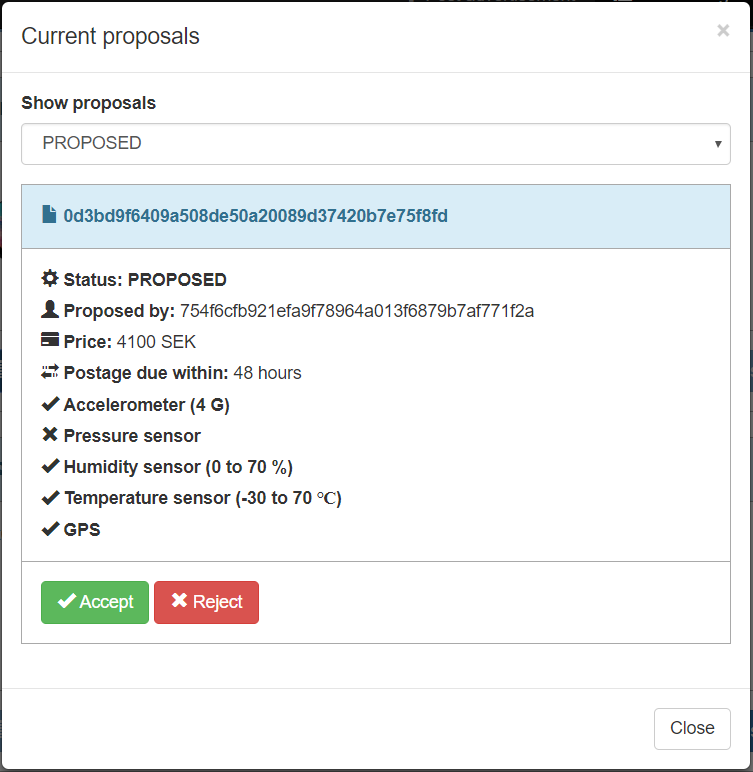
\includegraphics[scale=0.58]{app_screens/terms_accept.png}
\caption{Agreement terms modal.}
\label{fig:explorerdash}
\end{figure}

\subsubsection{Logistics process and simulation}

\paragraph{Step 1 - Initiation of the logistics process}

In order not to violate agreement terms, the item, for which an agreement was established, is required to be sent to the buyer, before the logistics timeout is reached (it is configured in the accepted terms). As mentioned before, the logistics process is simulated by the external simulator. In order to initiate the transfer of goods, the seller needs to provide agreement identifier to the logistics company employee, who then enters it into the corresponding field on the starting page of the simulator. Unique package number is then generated and all of the logistics parameters are automatically fetched from the agreement's terms. All of that information is displayed on the screen for the logistics company employee to see, in order to know what sensors to attach to the package and where to send it. Once that is done, the item is weighed, the seller pays for the transport and package is being sent to the buyer. It is important to know that buyer and seller never get to know eachother's private information, as it will only be visible to the logistics company staff.

\begin{figure}[H]
\centering
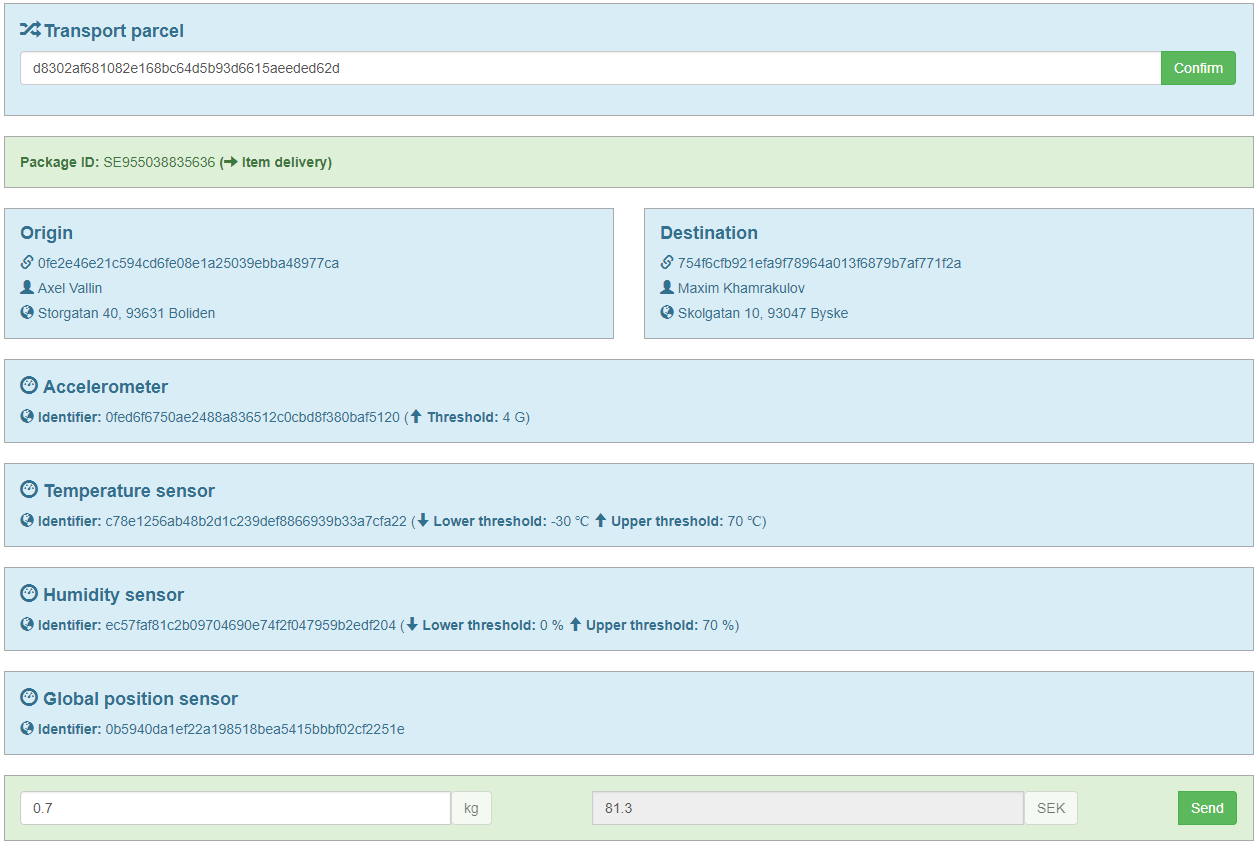
\includegraphics[scale=0.345]{app_screens/simulator_init.png}
\caption{Logistics initiation screen.}
\label{fig:siminit}
\end{figure}

\paragraph{Step 2 - Simulation of parcel transport}
Simulation process was described in Section \ref{section:simulation}. Simulator application supports transport in both directions (both from the seller to buyer and back, in case of return). Once the item is delivered, the buyer pays for the item and has 24 hours to leave feedback on the item's condition.

\begin{figure}[H]
\centering
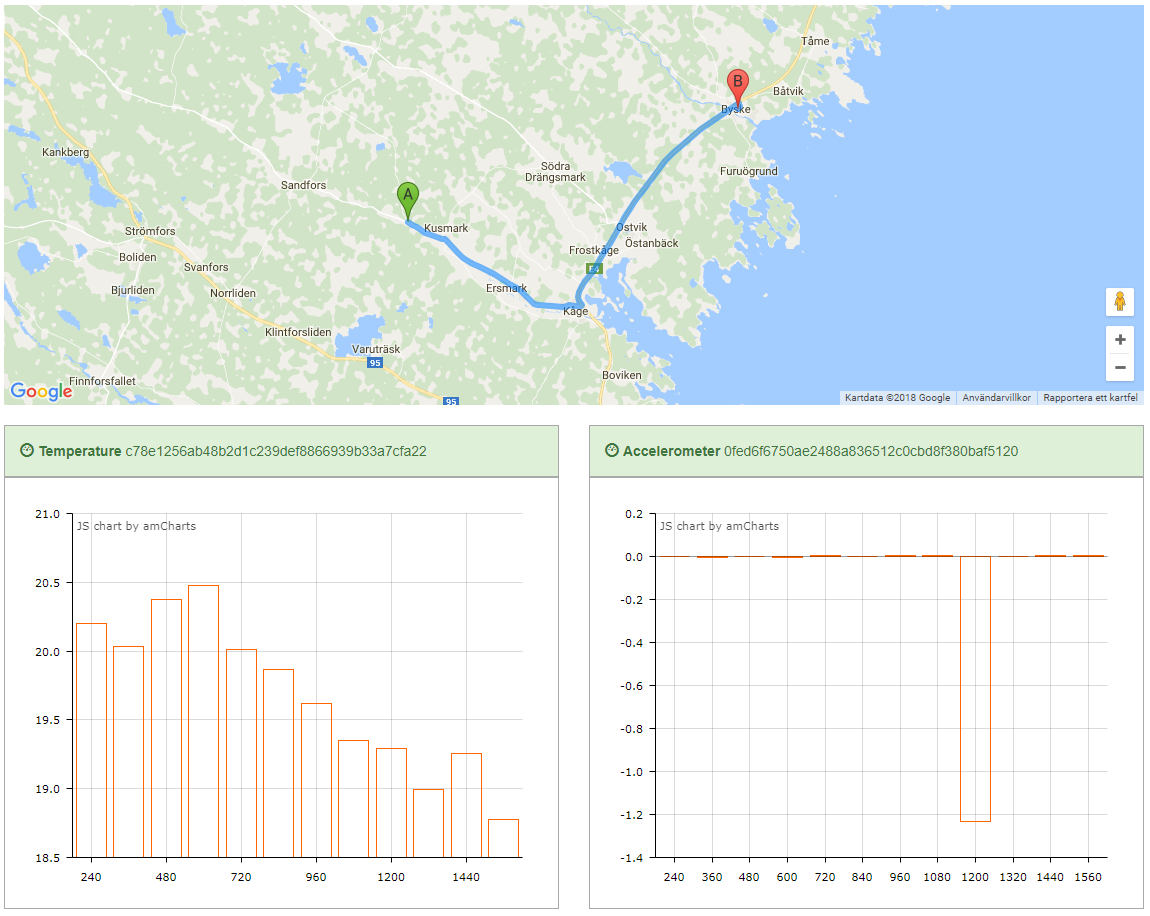
\includegraphics[scale=0.36]{app_screens/simulator_transport.png}
\caption{Part of the simulation process screen.}
\label{fig:simtransport}
\end{figure}

\subsubsection{Logistics process monitoring}

\paragraph{Step 1 - Locating the agreement}
Using the web interface, it is possible to monitor sensor outputs and see current position of the parcel (in case of GPS sensor being included), during the logistics process. In order to do that, the relevant agreement needs to be located. In case of the seller, this procedure was described in Section \ref{section:initiation}. In case of the buyer, the process is roughly the same apart from navigating to the "Bought items" submenu instead.

\paragraph{Step 2 - Displaying the agreement information screen}
Once the agreement is located, the users may click on it to navigate to the agreement information screen. General information about the item, its accepted terms and logistics monitoring is integrated in that module. Buyers and sellers are also able to accept and decline conditions of deliveries and returns respectively. Clerk decisions are also shown here, where applicable. Sensor readouts and map location can be toggled and hidden by clicking the buttons. Sensor readouts are visualized in form of charts. 

\begin{figure}[H]
\centering
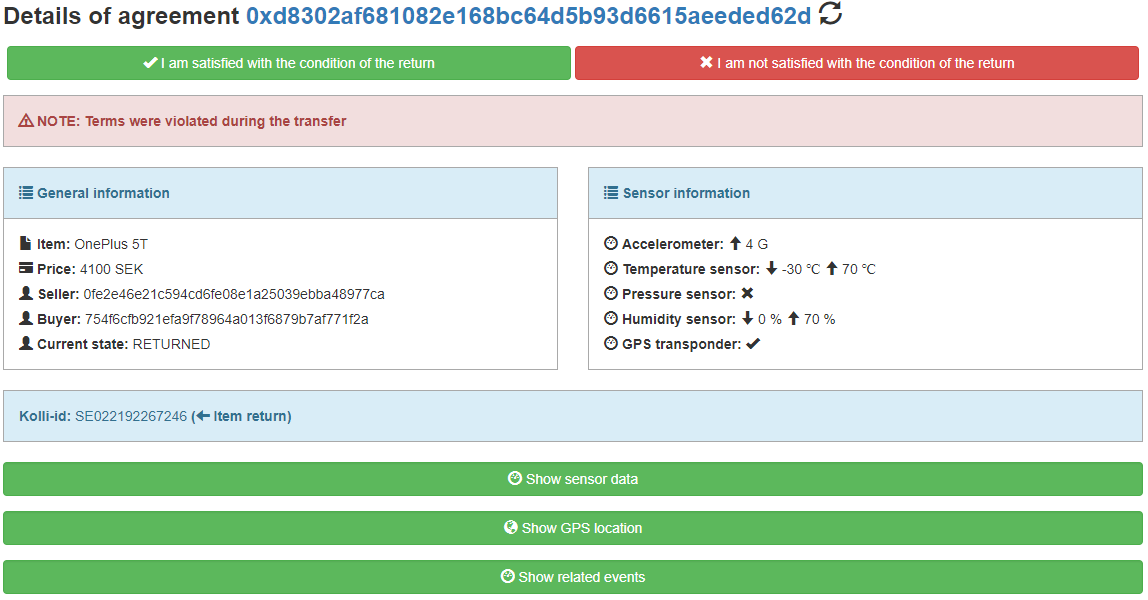
\includegraphics[scale=0.485]{app_screens/agreement_display.png}
\caption{Agreement information screen.}
\label{fig:agreementdisplay}
\end{figure}

\subsubsection{Exploring agreements}

\paragraph{Step 1 - Accessing the explorer dashboard}
The explorer module can be accessed without logging in to the application, as its goal is to be as transparent as possible. It is used to find out more detailed information about agreements, accounts terms, etc. The user is navigated to the explorer dashboard, if the corresponding button on the top navigation bar's left field is pressed. Explorer dashboard consists out of a search bar, recent agreements and recent events fields.

\begin{figure}[H]
\centering
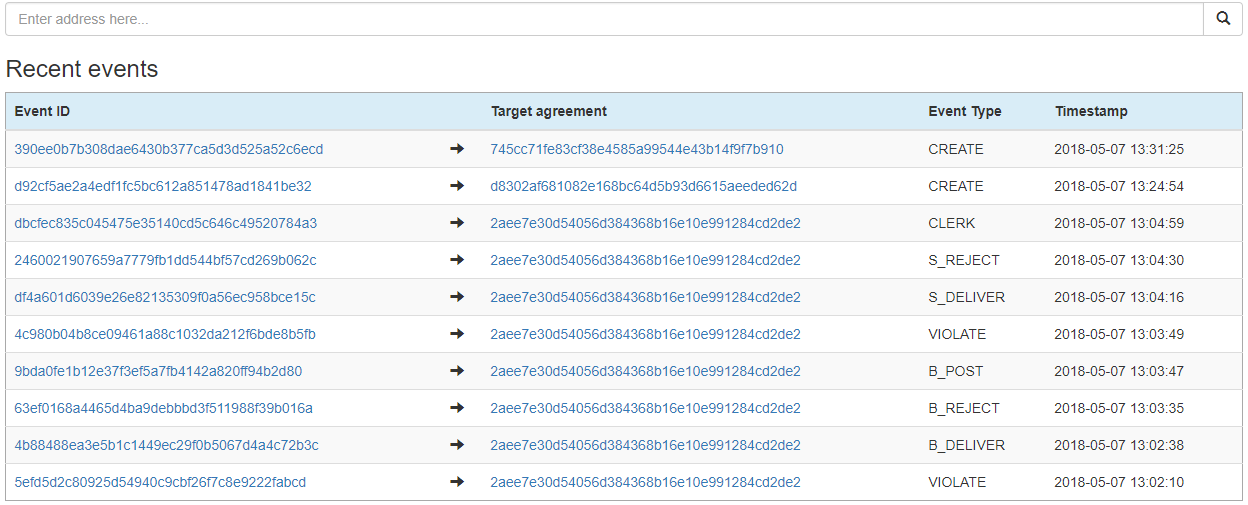
\includegraphics[scale=0.42]{app_screens/explorer_events.png}
\caption{Recent events display in the explorer screen.}
\label{fig:explorerdash}
\end{figure}

\paragraph{Step 2 - Explorer display}
In order to display information about an agreement, its unique identifier needs to by provided in the search bar. Once fetched, the agreement data is presented in JSON format. Additionally, the agreement-related events are represented in the table, which is located below the agreement data display.

\begin{figure}[H]
\centering
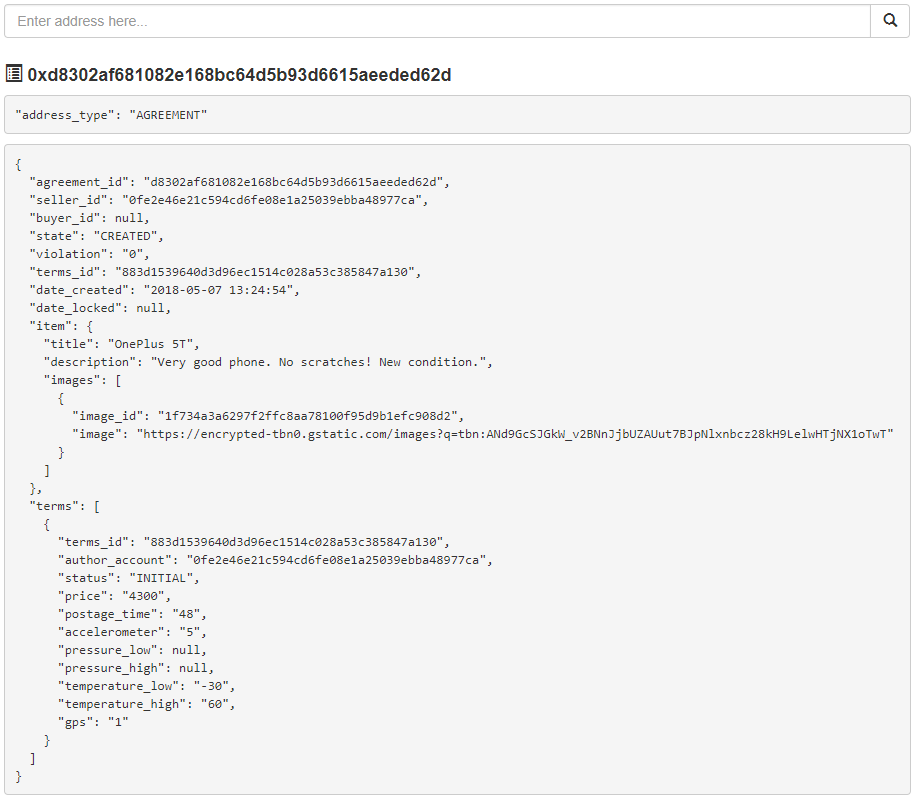
\includegraphics[scale=0.51]{app_screens/explorer_agreement.png}
\caption{Agreement data display. Data is represented in JSON format.}
\label{fig:exploreragreement}
\end{figure}

\subsubsection{Clerk resolving}

\paragraph{Step 1 - Logging in with clerk account and accessing the conflict request}

Conflict resolving is established by clerk administrators, who serve as notarius publicus. Conflict resolving module is accessed by clicking the corresponding button in the bottom navigation bar and is only available to clerk administrators, using special clerk accounts. The clerk dashboard page consists out of pending conflict requests and resolved conflicts tables.

\begin{figure}[H]
\centering
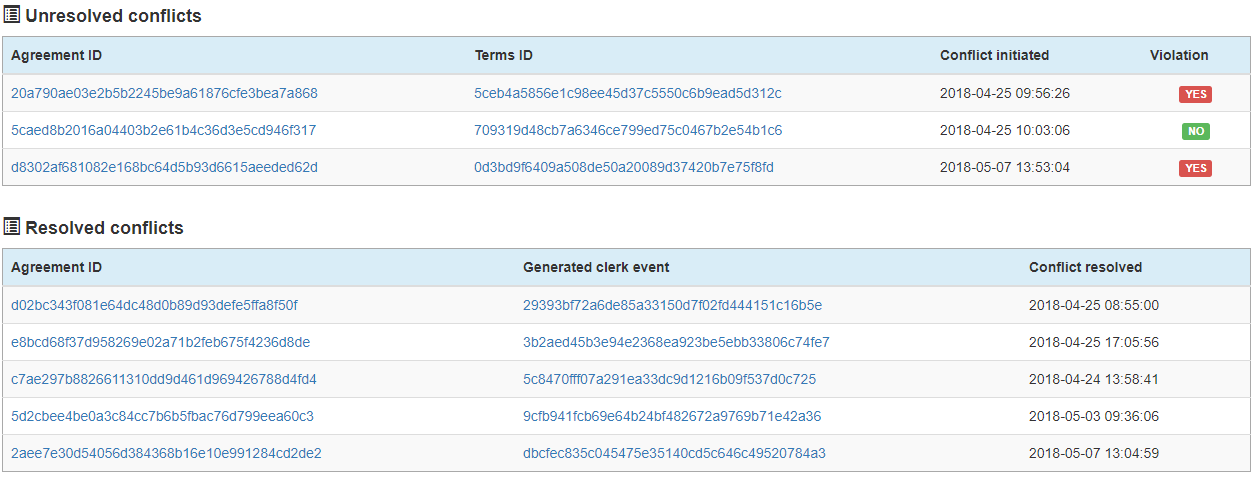
\includegraphics[scale=0.445]{app_screens/clerk_dash.png}
\caption{Clerk administrator dashboard.}
\label{fig:clerkdash}
\end{figure}

\paragraph{Step 2 - Conflict resolving dashboard}
In order to resolve a pending conflict, the clerk needs to click the corresponding column in the table. This redirects the clerk to the resolving dashboard. The dashboard contains all relevant information, which can be useful to the clerk, in order to accurately determine what party should be held responsible for the conflict. Information about transfer, return, as well as general information about the agreement and its terms is available to the clerk. Clerk's decision is meant to be final without any possibility of being reconsidered within the context of the Secure Package. Users have 24 hours to confirm clerk's decision, otherwise it is confirmed automatically. In case of decision not being accepted by either parties, a higher-order legal authority should be contacted.

\begin{figure}[H]
\centering
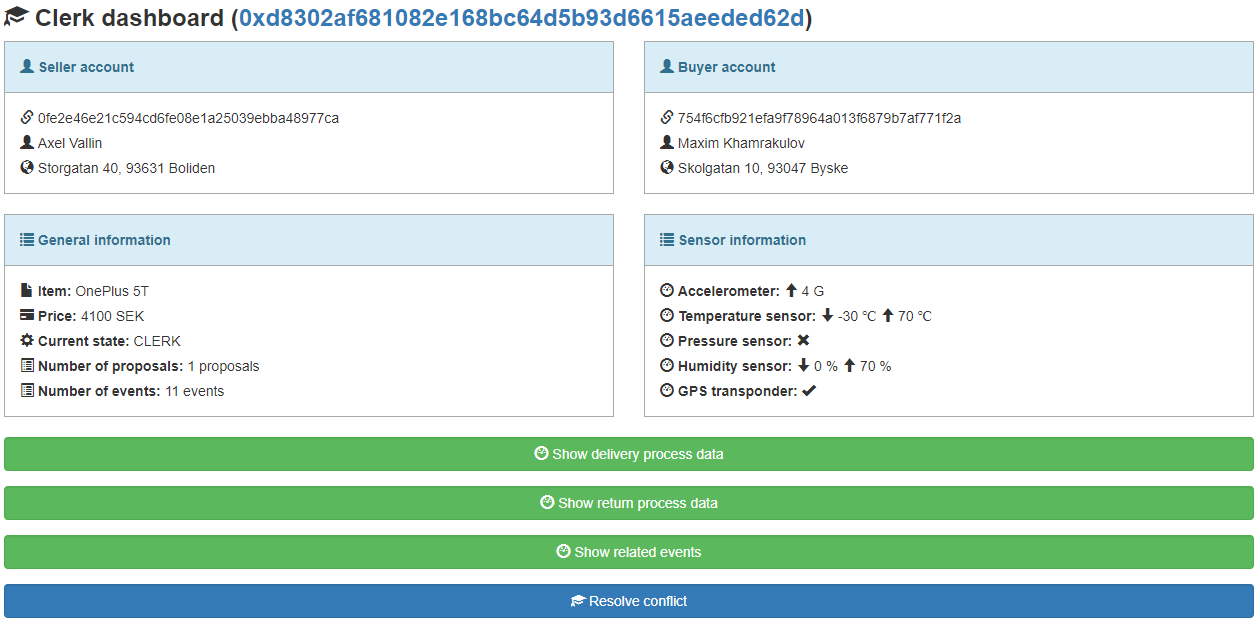
\includegraphics[scale=0.44]{app_screens/clerk_resolvement.png}
\caption{Clerk resolving screen.}
\label{fig:clerkresolvement}
\end{figure}

\subsubsection{Other user actions}
User actions, such as item history display, browsing of inactive proposals, removal of advertisements etc. were not described in this section, as they are very trivial and are not that important to consider in order to get an understanding of how the application works.